% ==============================================================================
% CAPITOLO 1: SCIENZA ECONOMICA ED ECONOMIA
% ==============================================================================
\chapter{Scienza Economica ed Economia}
\label{chap:scienza_economica}

\begin{tcolorbox}[colback=navyblue!5!white, colframe=navyblue, title=\textbf{Quadro Concettuale e Obiettivi Didattici}]
Il presente capitolo introduce l'architettura concettuale della scienza economica per l'ingegneria gestionale: il metodo scientifico (teoria, modello matematico ed evidenza empirica), i sei principi cardine del ragionamento economico (scarsità, costo opportunità, razionalità al margine, incentivi, vantaggi dello scambio, neutralità del mercato), il problema allocativo fondamentale, il ruolo del meccanismo dei prezzi e della "mano invisibile", le cause dei fallimenti del mercato e la distinzione epistemologica tra economia positiva ed economia normativa.
\end{tcolorbox}

\section{Metodologia dell'Apprendimento ed Economia per l'Ingegneria}

\subsection{Il Modello di Apprendimento Universitario vs Approccio d'Esame}
A livello universitario la conoscenza economica viene strutturata secondo un processo deduttivo-induttivo rigoroso:
\begin{equation}
    \textbf{Teoria Generale} \;\longrightarrow\; \textbf{Modello Matematico Rigoroso} \;\longrightarrow\; \textbf{Esempi ed Applicazioni}
\end{equation}
\begin{itemize}
    \item \textbf{Teoria}: corpus di proposizioni scientifiche astratte che spiegano i fenomeni;
    \item \textbf{Modello Matematico}: formalizzazione analitica semplificata che disciplina e quantifica le relazioni teoriche;
    \item \textbf{Esempi Applicativi}: casi reali che chiarificano e validano il modello.
\end{itemize}

\begin{figure}[htbp]
\centering
\begin{tikzpicture}[node distance=1.8cm, auto, >=Latex]
    \node [draw, rounded corners, fill=navyblue!10, text width=4.2cm, align=center, thick] (teoria) {\textbf{Teoria Economica}\\\small (Ipotesi astratte e principi)};
    \node [draw, rounded corners, fill=purpleaccent!10, text width=4.5cm, align=center, thick, right=1.5cm of teoria] (modello) {\textbf{Modello Matematico}\\\small (Equazioni, vincoli e funzioni)};
    \node [draw, rounded corners, fill=forestgreen!10, text width=4.2cm, align=center, thick, right=1.5cm of modello] (esempi) {\textbf{Applicazioni ed Esempi}\\\small (Casi reali ed evidenze)};
    
    \draw [->, ultra thick, color=navyblue] (teoria) -- node[above]{\footnotesize Formalizzazione} (modello);
    \draw [->, ultra thick, color=purpleaccent] (modello) -- node[above]{\footnotesize Risoluzione} (esempi);
    
    \draw [->, dashed, ultra thick, color=crimsonred] ($(esempi.south)+(0,-0.3)$) -- ++(0,-0.8) -| node[pos=0.25, below]{\textbf{Percorso d'Esame:} Esercizio $\to$ Modello $\to$ Teoria} ($(teoria.south)+(0,-0.3)$);
\end{tikzpicture}
\caption{Flusso logico dell'apprendimento teorico e percorso inverso nella risoluzione delle prove d'esame.}
\label{fig:apprendimento_economia}
\end{figure}

\begin{esame}[Percorso Logico d'Esame]
Mentre l'apprendimento teorico procede dalla teoria all'esempio, in sede di prova d'esame il ragionamento opera in senso strettamente inverso: si parte dal problema/esercizio quantitativo, si individua il modello matematico sottostante e si giustificano i passaggi risalendo alla teoria economica generale.
\end{esame}

\subsection{Perché Studiare Economia in Ingegneria Gestionale?}
Nell'ottica della figura professionale dell'ingegnere gestionale:
\begin{enumerate}
    \item \textbf{Evoluzione di Carriera}: dai compiti operativi e tecnici iniziali si passa progressivamente a ruoli direzionali caratterizzati da responsabilità decisionali crescenti;
    \item \textbf{Gestione delle Risorse e Budget}: ogni decisione di investimento, produzione, logistica o innovazione si scontra con risorse finanziarie, umane e temporali rigorosamente limitate;
    \item \textbf{Valore Aggiunto rispetto all'Automazione}: i compiti ripetitivi basati su risposte note vengono rapidamente delegati a strumenti automatici; le capacità insostituibili dell'ingegnere consistono nell'affrontare problemi inediti, strutturare modelli decisionali e compiere scelte strategiche in condizioni di incertezza.
\end{enumerate}

\subsection{Obiettivi Didattici e Rigore Lessicale}
L'analisi economica richiede una precisione lessicale assoluta:
\begin{itemize}
    \item \textbf{Ricavo}: flusso monetario lordo derivante dalla vendita di beni e servizi ($\RT = P \cdot Q$);
    \item \textbf{Costo}: valore monetario di tutte le risorse impiegate nel processo produttivo ($\CT$);
    \item \textbf{Profitto}: eccedenza netta dei ricavi rispetto ai costi complessivi ($\Pi = \RT - \CT$);
    \item \textbf{Reddito}: flusso monetario percepito da un individuo o fattore in un intervallo di tempo (salario, rendita, dividendo).
\end{itemize}

\begin{definizione}{Articolazione dell'Economia: Microeconomia e Macroeconomia}{micro_macro}
\begin{itemize}
    \item \textbf{Microeconomia}: studia i comportamenti decisionali dei singoli agenti economici (consumatori, lavoratori, singole imprese) e la struttura dei singoli mercati.
    \item \textbf{Macroeconomia}: studia il sistema economico a livello aggregato (PIL, livello generale dei prezzi, disoccupazione complessiva, moneta, bilancia dei pagamenti e politiche di governo).
\end{itemize}
\end{definizione}

\section{I Sei Principi Cardine del Ragionamento Economico}

La disciplina economica moderna si fonda su sei pilastri concettuali essenziali:

\subsection{1. Il Principio di Scarsità e il Concetto di Trade-off}

\begin{legge}{Principio di Scarsità}{principio_scarsita}
Una risorsa è \textbf{scarsa} quando, a un prezzo nullo, la quantità domandata eccede l'offerta disponibile. Poiché le risorse totali sono finite a fronte di bisogni illimitati, ogni scelta implica necessariamente un \textbf{trade-off}: per ottenere una quantità maggiore di un bene o servizio è indispensabile rinunciare a qualcos'altro.
\end{legge}

\begin{esempio}[Trade-off Quotidiani e Professionali]
\begin{itemize}
    \item \textit{Scelta Lavoro vs Tempo Libero}: un individuo che decide di lavorare ore supplementari ottiene un reddito monetario maggiore ma rinuncia al riposo, allo studio o allo svago;
    \item \textit{Scelta di Studio}: dedicare 4 ore allo studio di Economia implica rinunciare a studiare un'altra materia o a svolgere attività sportive.
\end{itemize}
\end{esempio}

\subsection{2. Il Principio del Costo Opportunità}

\begin{definizione}{Costo Opportunità}{costo_opportunita}
Il \textbf{costo opportunità} di una determinata scelta $A$ è il valore economico della migliore tra tutte le alternative scartate ($B, C, \dots$) a cui si è rinunciato:
\begin{equation}
    \text{Costo Opportunità}(A) = \max \{ \text{Valore}(B), \text{Valore}(C), \dots \}
\end{equation}
\end{definizione}

\begin{osservazione}[Costi Monetari vs Costi Economici Impliciti]
Il costo opportunità include sia le spese contabili dirette (costi espliciti) sia il valore dei mancati guadagni (costi impliciti).
\end{osservazione}

\begin{esempio}[Il Vero Costo dell'Università]
Qual è il costo complessivo di frequentare il corso di laurea in Ingegneria Gestionale a Pisa?
\begin{itemize}
    \item \textbf{Costi Espliciti (Monetari)}: tasse universitarie, libri di testo, trasporti, alloggio per studenti fuori sede;
    \item \textbf{Costi Impliciti (Costo Opportunità del Tempo)}: il salario netto a cui lo studente rinuncia non entrando immediatamente nel mercato del lavoro a tempo pieno dopo il diploma.
\end{itemize}
L'investimento in istruzione universitaria è economicamente razionale poiché il premio salariale futuro del laureato (differenziale retributivo lungo l'intero ciclo di vita lavorativa) compensa ampiamente la somma dei costi espliciti e del costo opportunità sostenuto.
\end{esempio}

\subsection{3. Il Principio di Razionalità e la Scelta al Margine}

\begin{definizione}{Razionalità Economica e Marginalismo}{razionalita_margine}
In economia si assume che gli agenti siano \textbf{razionali}: essi perseguono coerentemente un obiettivo ben definito (le famiglie massimizzano l'utilità, le imprese massimizzano il profitto) valutando costi e benefici al \textbf{margine}.

Un agente compie decisioni incrementali confrontando il \textbf{Beneficio Marginale} ($\mathrm{BMg}$) con il \textbf{Costo Marginale} ($\mathrm{CMg}$):
\begin{itemize}
    \item \textbf{Costo Marginale ($\mathrm{CMg}$)}: incremento del costo totale generato dallo svolgimento di una unità aggiuntiva di attività;
    \item \textbf{Beneficio Marginale ($\mathrm{BMg}$)}: incremento del beneficio (o ricavo) totale derivante dall'unità aggiuntiva.
\end{itemize}
\end{definizione}

\begin{metodo}[Regola di Ottimo al Margine]
L'agente razionale incrementa il livello di attività finché:
\begin{equation}
    \mathrm{BMg} \ge \mathrm{CMg}
\end{equation}
Il livello ottimo di attività $x^*$ è individuato dalla condizione di equilibrio marginale:
\begin{equation}
    \mathrm{BMg}(x^*) = \mathrm{CMg}(x^*)
\end{equation}
\end{metodo}

\begin{esame}[Tranello Tipico: Variabili Medie vs Variabili Marginali]
Uno degli errori più gravi e frequenti all'esame consiste nel confondere le grandezze medie con quelle marginali:
\begin{itemize}
    \item $\text{Costo Medio} = \frac{\text{Costo Totale}}{n}$ (costo unitario medio su tutte le unità già prodotte);
    \item $\text{Costo Marginale} = \CT(n+1) - \CT(n) = \dv{\CT}{n}$ (costo di realizzare l'unità successiva).
\end{itemize}
Le decisioni ottimali dipendono \textbf{esclusivamente dai valori marginali}, non da quelli medi.
\end{esame}

\begin{esempio}[Casi Reali di Decisioni al Margine]
\begin{enumerate}
    \item \textbf{Produzione d'Impresa}: se un impianto produce 100 componenti a un costo totale di 10.000\,\euro{} (costo medio = 100\,\euro{}), e la produzione della 101-esima unità richiede 60\,\euro{} extra di materie prime, il costo marginale è 60\,\euro{} (non 100\,\euro{}). Se il prezzo di vendita è 80\,\euro{}, l'impresa deve produrre l'unità addizionale poiché $\mathrm{BMg} = 80 > \mathrm{CMg} = 60$.
    \item \textbf{Rifiuto di un Voto d'Esame}: uno studente che ha la media del 28 e riceve 24 all'ultimo esame valuta il beneficio marginale (il voto 24 incrementa il numero di crediti ma riduce la media finale) rispetto al costo marginale (ripetere l'esame, tempo e stress). Se l'obiettivo è massimizzare la media per la borsa di studio, il voto viene rifiutato.
    \item \textbf{Confezioni al Supermercato}: la scelta tra la bottiglia singola e il multipack di Coca-Cola richiede di confrontare la differenza di prezzo marginale con la quantità aggiuntiva effettivamente consumabile prima della scadenza.
    \item \textbf{La Sveglia al Mattino}: dormire 15 minuti in più apporta un beneficio marginale decrescente di riposo, ma genera un costo marginale crescente (dover fare colazione di fretta, rischiare il ritardo al lavoro o nel traffico).
\end{enumerate}
\end{esempio}

\subsection{4. Il Principio degli Incentivi}

\begin{legge}{Reattività agli Incentivi}{principio_incentivi}
Gli agenti economici modificano sistematicamente il proprio comportamento al variare dei costi e benefici marginali. Un \textbf{incentivo} è qualunque variazione esogena che incrementa il beneficio marginale o riduce il costo marginale di una scelta.
\end{legge}

\begin{esempio}[Perché il Cibo sui Voli di Linea è spesso Mediocre?]
Un passeggero desidererebbe consumare un pasto di alta cucina a bordo di un aereo. Tuttavia:
\begin{itemize}
    \item La disponibilità a pagare per un pasto eccellente in volo è contenuta (es. 5--10\,\euro{});
    \item Preparare cibo espresso a bordo richiederebbe l'installazione di forni professionali, cucine dedicate e personale qualificato, eliminando file di sedili;
    \item La compagnia aerea dovrebbe spalmare i mancati ricavi dei biglietti persi sul prezzo del volo (costo marginale di circa 50--80\,\euro{} a passeggero).
\end{itemize}
Poiché il costo marginale del servizio ($50$\,\euro{}) supera ampiamente il beneficio marginale percepito dal viaggiatore ($10$\,\euro{}), la compagnia razionale sceglie di offrire pasti precotti semplici, mantenendo il biglietto aereo a tariffe competitive.
\end{esempio}

\begin{esempio}[Incentivi Economici e Politica Pubblica]
\begin{itemize}
    \item \textit{Scelta Universitaria}: l'aumento delle retribuzioni relative per gli ingegneri gestionali rispetto ad altri settori induce un incremento delle immatricolazioni a tale corso di laurea;
    \item \textit{Prezzo dei Carburanti}: una tassa ecologica sulla benzina incentiva l'acquisto di veicoli elettrici, l'uso del trasporto pubblico e la mobilità dolce;
    \item \textit{Piano Transizione 4.0}: crediti d'imposta sugli investimenti in macchinari digitali e interconnessi riducono il costo del capitale, stimolando l'ammodernamento industriale.
\end{itemize}
\end{esempio}

\subsection{5. Il Principio dei Vantaggi dello Scambio (Gains from Trade)}

\begin{teorema}{Specializzazione e Vantaggi dello Scambio}{vantaggi_scambio}
Lo scambio volontario non è un gioco a somma zero, bensì genera un beneficio netto per tutte le parti coinvolte. La specializzazione dei singoli individui (e delle nazioni) nelle attività in cui godono di un \textbf{vantaggio comparato} massimizza la produzione aggregata totale e il consumo complessivo.
\end{teorema}

\begin{esempio}[Il Manager e il Giardiniere]
Supponiamo che un ingegnere impieghi 1 ora per redigere una complessa relazione tecnica e 1 ora per potare il giardino di casa. Un giardiniere professionista impiega 3 ore per la relazione tecnica e 20 minuti per potare il giardino.
Anche qualora l'ingegnere fosse più rapido del giardiniere in entrambe le mansioni, all'ingegnere conviene concentrarsi esclusivamente sulla relazione tecnica (dove la sua produttività oraria monetaria è massima) e remunerare il giardiniere per la cura del verde. Entrambi ottengono una dotazione finale superiore a quella di autosufficienza.
\end{esempio}

\subsection{6. Il Principio della Neutralità del Mercato e i suoi Limiti}

\begin{definizione}{Neutralità del Mercato}{neutralita_mercato}
Nella teoria economica neoclassica standard, il mercato è assunto come un'istituzione \textbf{neutrale}: esso alloca beni e servizi in base alla disponibilità a pagare senza alterare le preferenze, i valori etici o le motivazioni intrinseche degli individui.
\end{definizione}

\begin{osservazione}[Critica della Neutralità: Il Caso delle Donazioni di Sangue]
L'evidenza empirica mostra che talvolta l'introduzione di incentivi monetari in ambiti regolati da norme sociali o altruismo può produrre effetti perversi (\textit{crowding out} delle motivazioni intrinseche):
\begin{itemize}
    \item In Italia la donazione di sangue è gratuita e volontaria, considerata un dovere civico e di solidarietà;
    \item In alcuni contesti esteri in cui è stata introdotta una remunerazione in denaro per ogni donazione, il numero complessivo di donatori è paradossalmente diminuito: la retribuzione ha trasformato un gesto nobilmente etico in una transazione commerciale, allontanando i donatori altruisti.
\end{itemize}
\end{osservazione}

\begin{figure}[htbp]
\centering
\begin{tikzpicture}[scale=0.9]
    \node[draw, fill=navyblue!15, rounded corners, inner sep=6pt, align=center, thick] (scarsita) at (0,4) {\textbf{1. Scarsità}\\\small Risorse finite, trade-off};
    \node[draw, fill=navyblue!15, rounded corners, inner sep=6pt, align=center, thick] (costo) at (5.5,4) {\textbf{2. Costo Opportunità}\\\small Valore della migliore alternativa};
    \node[draw, fill=purpleaccent!15, rounded corners, inner sep=6pt, align=center, thick] (razionalita) at (11,4) {\textbf{3. Razionalità al Margine}\\\small Confronto $\mathrm{BMg}$ vs $\mathrm{CMg}$};
    
    \node[draw, fill=purpleaccent!15, rounded corners, inner sep=6pt, align=center, thick] (incentivi) at (0,0) {\textbf{4. Incentivi}\\\small Reazione ai costi/benefici};
    \node[draw, fill=forestgreen!15, rounded corners, inner sep=6pt, align=center, thick] (scambio) at (5.5,0) {\textbf{5. Vantaggi Scambio}\\\small Specializzazione e divisione lavoro};
    \node[draw, fill=forestgreen!15, rounded corners, inner sep=6pt, align=center, thick] (neutralita) at (11,0) {\textbf{6. Neutralità Mercato}\\\small Interazione prezzi e valori};
    
    \draw[->, thick, color=navyblue] (scarsita) -- (costo);
    \draw[->, thick, color=navyblue] (costo) -- (razionalita);
    \draw[->, thick, color=purpleaccent] (razionalita) -- (incentivi);
    \draw[->, thick, color=forestgreen] (incentivi) -- (scambio);
    \draw[->, thick, color=forestgreen] (scambio) -- (neutralita);
\end{tikzpicture}
\caption{Rappresentazione organica dei sei principi cardine della scienza economica.}
\label{fig:sei_principi}
\end{figure}

\section{Il Problema Allocativo e i Sistemi Economici}

\subsection{Le Tre Domande Fondamentali}
Ogni collettività deve risolvere il cosiddetto \textbf{problema allocativo}:
\begin{enumerate}
    \item \textbf{Cosa e quanto produrre?} Quali beni e servizi realizzare e in quale quantità quantitativa;
    \item \textbf{Come produrre?} Con quali tecniche tecnologiche e combinazioni di fattori produttivi ($K$ e $L$);
    \item \textbf{Per chi produrre?} Come distribuire il reddito e i beni finali generati tra i cittadini.
\end{enumerate}

\subsection{Sistemi Economici a Confronto: Pianificazione vs Libero Mercato}

\begin{table}[htbp]
\centering
\small
\renewcommand{\arraystretch}{1.3}
\begin{tabularx}{\textwidth}{lXX}
\toprule
\textbf{Caratteristica} & \textbf{Economia Centralizzata (Pianificata)} & \textbf{Economia Decentrata (Libero Mercato)} \\
\midrule
\textbf{Soggetto Decisore} & Autorità centrale di pianificazione (Stato/Ministero) & Singoli consumatori e imprese autonome \\
\textbf{Coordinamento} & Direttive burocratiche e piani quantitativi obbligatori & Meccanismo dei prezzi di mercato liberi \\
\textbf{Proprietà Fattori} & Pubblica e statale dei mezzi di produzione & Privata dei mezzi di produzione e capitali \\
\textbf{Limiti Strutturali} & Deficit informativo, lentezza, inefficienza allocativa & Instabilità ciclica, disuguaglianze, fallimenti di mercato \\
\bottomrule
\end{tabularx}
\caption{Confronto istituzionale tra economia pianificata ed economia di mercato.}
\label{tab:sistemi_economici}
\end{table}

\section{Il Ruolo del Mercato, dei Prezzi e la Mano Invisibile}

\begin{definizione}{Mercato e Prezzo di Mercato}{mercato_prezzo}
Il \textbf{mercato} è l'insieme delle interazioni e delle istituzioni attraverso cui acquirenti e venditori di un bene o servizio entrano in contatto per determinare il prezzo e la quantità scambiata.

Il \textbf{prezzo di mercato} è il vettore informativo primario del sistema economico:
\begin{itemize}
    \item Trasmette istantaneamente informazioni sulla scarsità relativa del bene ai produttori e sull'intensità del bisogno ai consumatori;
    \item Raziona la domanda aggregata indirizzandola verso i consumatori che le attribuiscono maggior valore;
    \item Alloca le risorse produttive verso i settori a più alta redditività.
\end{itemize}
\end{definizione}

\begin{esempio}[Il Segnale del Prezzo del Caffè al Bar]
Consideriamo il prezzo di una tazzina di espresso al bar a 1,10\,\euro{}:
\begin{itemize}
    \item Dal lato della domanda, l'acquisto attesta che il beneficio marginale del consumatore è almeno pari a 1,10\,\euro{};
    \item Dal lato dell'offerta, il barista copre i costi marginali di miscela, energia, affitto e lavoro, ottenendo una congrua remunerazione del capitale investito;
    \item Se il prezzo salisse bruscamente a 10\,\euro{}, i consumatori ridurrebbero il consumo sostituendolo con preparazioni domestiche, costringendo i baristi a ribassare il prezzo;
    \item Se il prezzo scendesse a 0,10\,\euro{}, i locali andrebbero in perdita e chiuderebbero, creando penuria finché il prezzo non risalisse al valore di equilibrio sostenibile.
\end{itemize}
\end{esempio}

\begin{teorema}{La Mano Invisibile di Adam Smith (1776)}{mano_invisibile}
Nell'opera fondamentale \textit{"Indagine sulla natura e le cause della ricchezza delle nazioni"}, Adam Smith postulò che ciascun individuo, perseguendo razionalmente il proprio interesse personale ed economico privato, viene guidato da una \textbf{"mano invisibile"} a promuovere un fine che non era parte delle sue intenzioni: il benessere materiale e l'efficienza complessiva dell'intera società.
\end{teorema}

\begin{figure}[htbp]
\centering
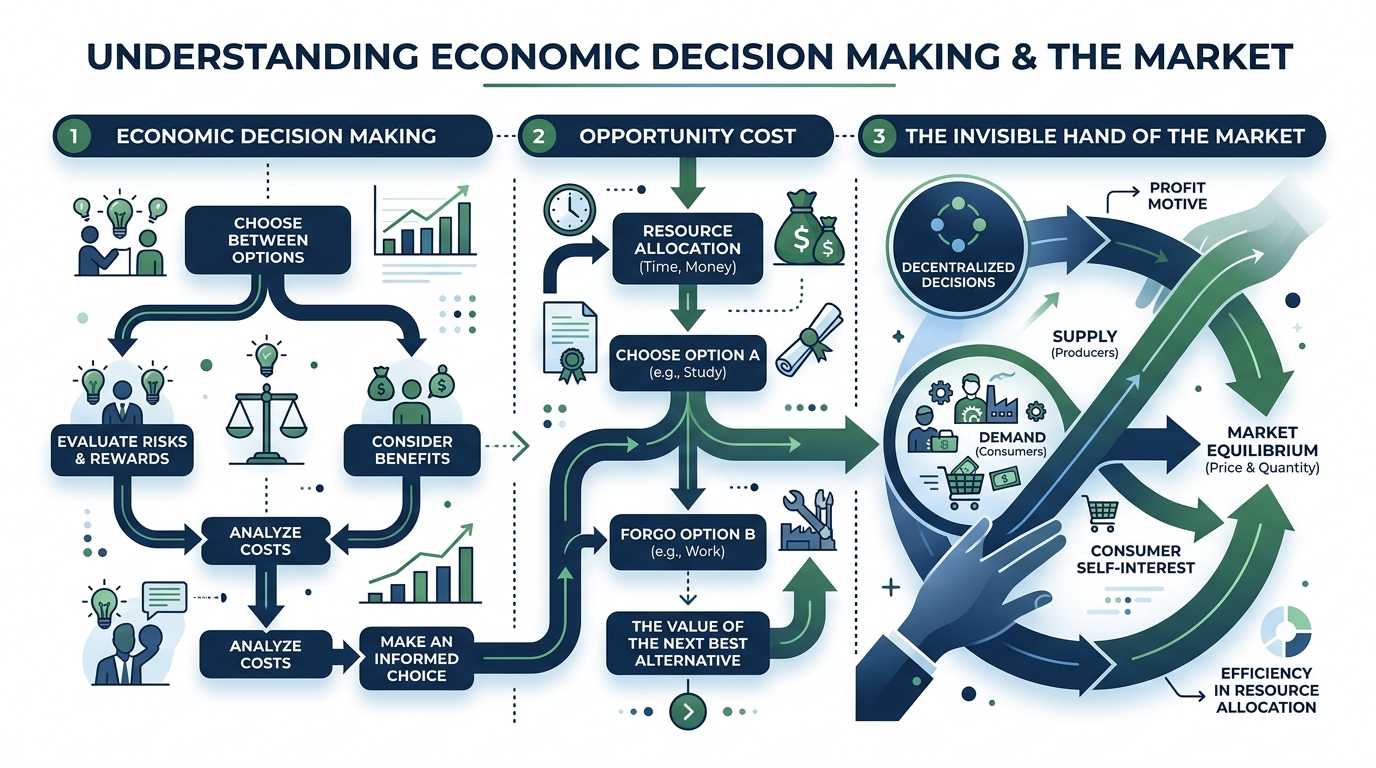
\includegraphics[width=0.92\textwidth]{figures/market_coordination_concept.jpg}
\caption{Rappresentazione concettuale del processo decisionale economico: costo opportunità, allocazione delle risorse e coordinamento di mercato guidato dalla mano invisibile.}
\label{fig:market_coordination}
\end{figure}

\section{I Fallimenti del Mercato e l'Economia Mista}

Sebbene il mercato sia uno strumento straordinario di coordinamento, esso non garantisce automaticamente l'ottimo sociale in presenza di \textbf{fallimenti del mercato}:

\subsection{Tassonomia dei Fallimenti del Mercato}

\begin{enumerate}
    \item \textbf{Esternalità}: effetti diretti dell'azione di un agente economico sul benessere di altri soggetti non coinvolti nella transazione, senza che vi sia un compenso monetario:
    \begin{itemize}
        \item \textbf{Esternalità Negative}: inquinamento industriale, congestione del traffico stradale, emissioni nocive (il costo privato è inferiore al costo sociale complessivo);
        \item \textbf{Esternalità Positive}: ricerca scientifica di base (es. gli studi di matematica pura applicati alle telecomunicazioni e alla meteorologia), vaccinazioni di massa, istruzione (il beneficio sociale è superiore al beneficio privato).
    \end{itemize}
    
    \item \textbf{Potere di Mercato e Monopolio}: quando una o poche grandi imprese controllano l'offerta, esse alzano i prezzi al di sopra del costo marginale ($P > \CMg$), riducendo la quantità scambiata e generando una perdita secca per la collettività.
    
    \item \textbf{Beni Pubblici Puri}: beni caratterizzati da:
    \begin{itemize}
        \item \textbf{Non-rivalità nel consumo}: il consumo da parte di un individuo non riduce la disponibilità per gli altri;
        \item \textbf{Non-escludibilità}: è tecnicamente o economicamente impossibile impedire la fruizione a chi rifiuta di pagare (fenomeno del \textit{free-riding}).
    \end{itemize}
    \textit{Esempi}: difesa nazionale, illuminazione pubblica, tutela dell'ordine pubblico, segnalazione marittima (fari).
    
    \item \textbf{Asimmetrie Informative}: situazioni in cui compratori e venditori non dispongono delle medesime informazioni sulle caratteristiche del bene o sul comportamento della controparte (selezione avversa e azzardo morale).
\end{enumerate}

\begin{definizione}{Economia Mista}{economia_mista}
L'\textbf{economia mista} è il modello economico adottato da tutti i moderni paesi industrializzati: la maggior parte delle attività produttive è affidata all'iniziativa privata e al mercato, mentre lo Stato interviene con la spesa pubblica, la tassazione, la regolamentazione antitrust e le aziende pubbliche per correggere i fallimenti di mercato, garantire la fornitura di beni pubblici e ridistribuire le risorse secondo principi di equità sociale.
\end{definizione}

\section{Economia Positiva ed Economia Normativa}

\begin{definizione}{Economia Positiva vs Normativa}{positiva_normativa}
\begin{itemize}
    \item \textbf{Economia Positiva}: branca descrittiva e causale che spiega oggettivamente il funzionamento economico attraverso proposizioni analitiche verificabili empiricamente (\textit{"se la banca centrale alza i tassi, gli investimenti diminuiscono"}).
    \item \textbf{Economia Normativa}: branca prescrittiva che formula giudizi di valore soggettivi, etici e politici sulle soluzioni desiderabili (\textit{"il governo deve ridurre le disuguaglianze aumentando le imposte sui grandi patrimoni"}).
\end{itemize}
\end{definizione}

\begin{esame}[Checklist d'Esame: Riconoscimento Enunciati]
\begin{itemize}
    \item Contiene criteri di giudizio etico ("dovrebbe", "è giusto", "è inaccettabile")? $\implies$ \textbf{Normativa}.
    \item È formulata come un'ipotesi di causa-effetto verificabile con i dati statistici? $\implies$ \textbf{Positiva}.
\end{itemize}
\end{esame}
